\documentclass[a4paper,12pt,titlepage]{article}
\usepackage{palatino}
\usepackage{graphicx}
\usepackage{float}
\usepackage{amsmath}
\usepackage{caption}
\usepackage{subcaption}
\usepackage[margin=1.5cm,includefoot]{geometry}
\usepackage[utf8]{inputenc}
\usepackage{hyperref}
\usepackage{url}
\usepackage{listings}
\usepackage{xcolor}


\renewcommand*{\familydefault}{\sfdefault}
\usepackage[portuguese]{babel}


\begin{document}

\section{Introdução}	
	O uso da tecnologia RFID está em crescente expansão, principalmente em aplicações de Supply Chain Management (SCM), no qual saber a localização de cada item da cadeia produtiva é crucial para garantir maior eficácia e eficiência de todo um sistema. Devido essa crescente adoção do RFID, fica constatado que o surgimento de um conjunto de normas que visem à padronização das tecnlogias usadas seria algo natural de se acontecer. Imagine a situação em que uma grande empresa do setor de varejo se funda com outra do mesmo setor, sendo que ambas usam RFID para a localização dos produtos. Se, por exemplo, o formato das TAGs utlizadas pelas empresas forem diferentes, já teremos uma enorme dificuldade de integrar as informações oriundas de cada sistema. Para evitar esse tipo de problema, existe o \textbf{GS1}.
	
	O GS1 é uma organização internacional neutra e sem fins lucrativos, que desenvolve e mantém padrões para cadeias de demanda e suprimentos de diversos setores produtivos. Ele atua principalmente nas áreas de bens do consumo e varejo, saúde e transporte e logística. Algumas empresas que trabalham com o GS1 são: Carrefour, amazon, Google e Coca Cola. 	
	O GS1 foi fundado na década de 70 pelos líderes da indústria dos EUA, tendo com sua primeira atividade a criação do padrão de código de barras conhecido como \textbf{GS1 barcode}, o qual é largamente utilizado até hoje. Com os avanços da tecnologia e seu crescente uso, em 2004 o GS1 criou o primeiro padrão para o RFID.

\section{Como funciona}
	O padão GS1 é divido em três grupos: Identificar, Capturar e Compartilhar. 
	\begin{figure}[h!]
		\centering
		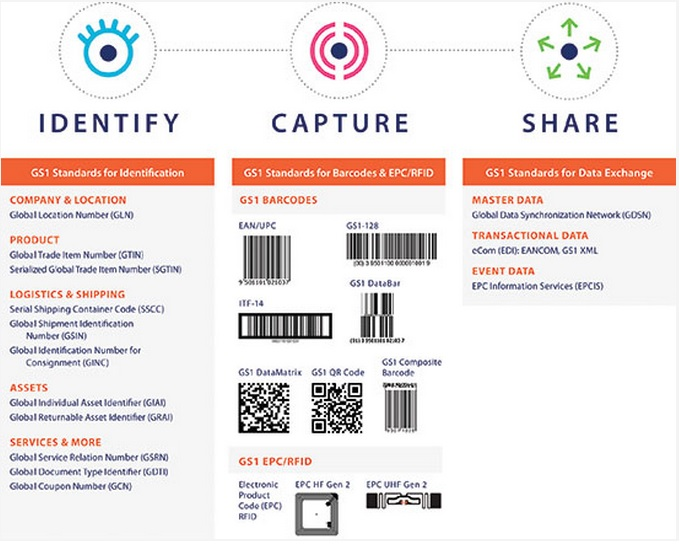
\includegraphics[width=0.7\linewidth]{gs1arch}
		\caption{Arquitetura do GS1}
		\label{fig:gs1arch}
	\end{figure}

	\paragraph{Identificar} Define códigos de identificação únicos que podem ser usados por um sistema de informação para se referir sem ambiguidade a qualquer tipo de produto.
	\paragraph{Capturar} Inclui definições de códigos de barra e RFID, além de especificar padrões para interfaces entre os elementos de software e hardware que se conectam às aplicações empresariais.
	\paragraph{Compartilhar} Define padrões para o formato dos dados trocados entre as aplicações e os clientes.     

\section{EPCGlobal}
	O padrão ECPglobal é uma iniciatia do GS1 para desevolver padrões voltados à indústria para o EPC, com o objetivo de dar suporte ao uso de RFID. Ele é divido em duas partes: \textbf{EPC/RFID} Tags e \textbf{EPCIS}. 
	
	O EPC (Electronic Product Code) é responsável por interligar o mundo do RFID com os códigos de barra do padrão GS1. Isso funciona da seguinte forma:
		\begin{figure}[h!]
			\centering
			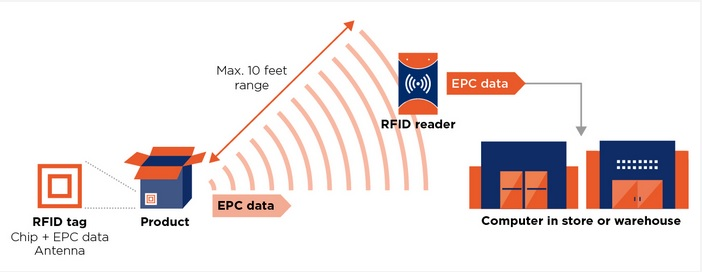
\includegraphics[width=0.7\linewidth]{epcrfid}
			\caption{Funcionamento do EPC}
			\label{fig:epcrfid}
		\end{figure}
	
	Capa produto contém um chip de memória contendo um EPC, o qual consiste de um número de série único. Em cada chip também há uma antena de rádio que transmite o ECP para um leitor RFID quando requisitado. Os dados capturados pelo leitor são então disponibilizados para os outros sistemas.
	
	% Falar sobre o EPCIS
	O EPCIS (Electronic Product Code Information Services) é o padrão que habilita as empresas parceiras a compartilhar informação sobre o movimento físico e status dos produtos enquanto eles trafegam pela linha de suprimentos. Uma vez que os dados EPC são coletados, como na figura \ref*{fig:epcrfid}, eles são disponibilizados à camada de negócios e todos que possuem acesso a este podem saber o histórico de movimento dos produtos. 
	\begin{figure}[h!]
		\centering
		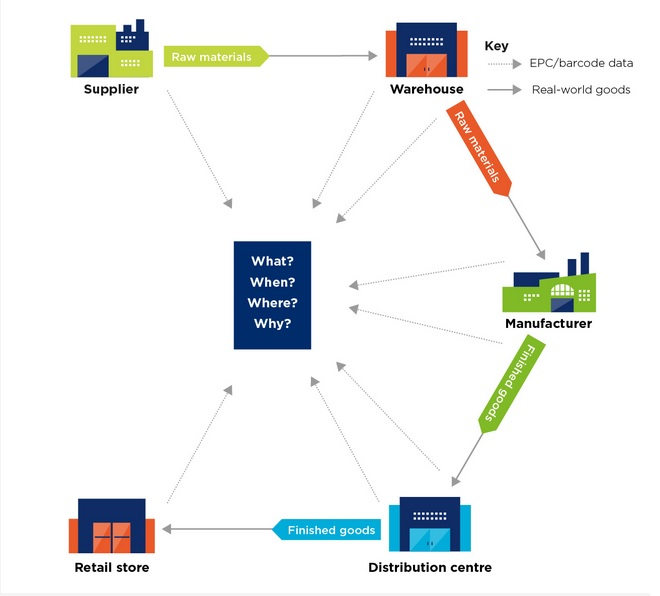
\includegraphics[width=0.7\linewidth]{epcis}
		\caption{Funcionamento do EPCIS}
		\label{fig:epcrfid}
	\end{figure}
		
\end{document}